\documentclass[12pt,a4paper]{article}
\usepackage{preamble}
\let\AltKey=\Alt
\let\Alt=\relax
\usepackage{menukeys}
\newcommand\sessiontitle{Lab Session 1}
\newcommand\sessionsubtitle{Python introduction and Jupyter notebooks}

%%%%%%%%%%%%%%%%%%%%%%%%%%%%%%%%%%%%%%%%%%
\begin{document}

\begin{description}
\item[Course web-page:]~\\\url{https://github.com/BMCV/mobi-fs3-python/blob/master/README.md}
\item[Overview of running GitHub Codespaces:] \url{https://github.com/codespaces}
\end{description}

\section{Setting up your GitHub repository}
\label{task:preparation}
\begin{enumerate}
\item Open the course web-page in any web-browser of your choice.
\item Click on the ``Create a new repository from this template'' link.
\item This will load another web-page entitled ``Create a new repository''. Leave everything on default and confirm the creation of the repository by clicking the ``Create repository'' button.
\item You should see a ``Generating your repository'' message for a few seconds and then be presented with an \textbf{overview of your repository}. You just created your first GitHub repository -- congrats! :)
\end{enumerate}

\section{Firing up a GitHub Codespace}
\label{task:codespaces}
\begin{enumerate}
\item Open the \textbf{overview of your repository} on GitHub. This is the web-page that you landed on after completing Task~\ref{task:preparation}.
\item Click on the green ``Code`'' button, then select the ``Codespaces'' tab.
\item Click the green ``Create codespace on master'' button. This will load \textbf{VS Code} (Visual Studio Code) inside of your web-browser. Wait until everything is loaded, it may take about one minute.
\end{enumerate}

\begin{figure}[h!]
    \centering
    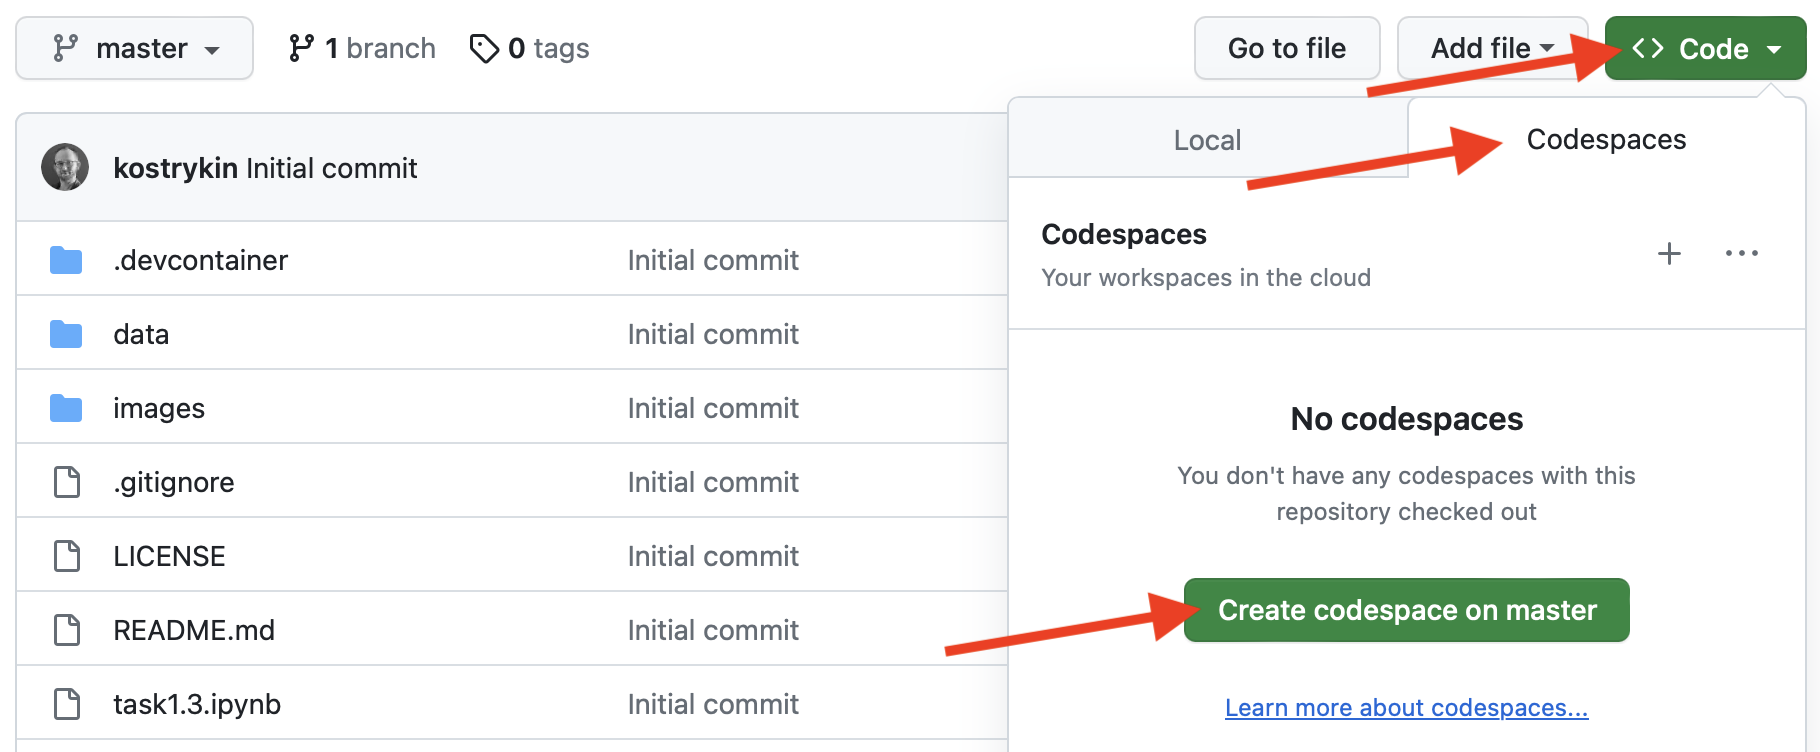
\includegraphics[width=0.7\textwidth]{images/codespaces.png}
\end{figure}

\textbf{Note:} If, at any time, \textbf{VS Code} behaves weirdly (e.g., complaining about missing extensions, not loading notebooks, or similar), try to simply reload the \textbf{VS Code} window. To do that, press \Ctrl+\keystroke{\shift}+\keystroke{P} (or \keystroke{\cmd}+\keystroke{\shift}+\keystroke{P} if you are on macOS) and type ``Reload window \Return''. Your work progress will be preserved.

\section{Your first Jupyter notebook}
The left panel of \textbf{VS Code} shows an overview of \textbf{your local repository}. Right now it is identical to your GitHub repository (which is the \textbf{origin} of your local repository). The assignments of this course are organized into several Jupyter notebooks. These are the "task*.ipynb" files that you can see in your repository. By progressing from task to task, you will have to work with different notebooks.

\begin{enumerate}
\item Double click the file "task1.3.ipynb" inside of \textbf{VS Code} to open the notebook for this task, and follow the instructions inside the notebook. -- \textbf{Note:} In Jupyter notebooks, code cells can be run in an \emph{arbitrary order}. This is very helpful for experimenting and trying out new things. Nevertheless, an assignment in this course is \emph{only} considered ``finished'' when the results can be reproduced by re-running all code cells \emph{from top to bottom} by clicking the ``Run all'' button.
\item When finished, close your notebook. Changes are saved automatically within \textbf{your local repository}, but remember, that those changes will be lost when you close the codespace, unless you push them to your GitHub repository.
\item To do that, click on the ``Terminal'' tab at the bottom of \textbf{VS Code} and type the following Git commands. -- \textbf{Hint:} The Git commands are given one per line, press \Return at the end of each command:
\begin{Verbatim}[frame=single]
git commit --all
git push origin master
\end{Verbatim}
Pressing \Return after the first command will open a text editor for typing a \textbf{commit message}. Type something like ``Finish task 1.3'' and close the editor.

The \textbf{commit message} is arbitrary. If you wanted, you could revert to any previous commit at a later time, and choosing an expressive message is convenient for finding the commit which you will be looking for. Besides, there are some conventions for how a \textbf{commit message} should be formatted: It should tell in an ``imperative mood'' and as concisely as possible, what \emph{the commit} should do\footnote{From the official Git documentation: \texttt{https://git.kernel.org/pub/scm/git/git.git/tree\\/Documentation/SubmittingPatches?h=v2.36.1\#n181}}.
\end{enumerate}

\section{Writing loops in Python}
Now you already know how to edit, commit, and push a Jupyter notebook.
\begin{enumerate}
    \item Open the notebook \texttt{task1.4.ipynb} and follow the instructions in the notebook.
    \item Commit and push your changes, then close \textbf{VS Code}.
\end{enumerate}
\end{document}
